\documentclass[aspectratio=169]{beamer}

\usepackage{ccicons}
\usepackage{fontspec}
\usepackage{listings}
\usepackage{tikz}
\usepackage{svg}

\definecolor{uclablue}{RGB}{39,116,174}
\definecolor{uclagold}{RGB}{255,179,0}

\definecolor{ubcorange}{RGB}{158, 66, 37}

\definecolor{cugold}{RGB}{207, 184, 124}
\definecolor{cudarkgray}{RGB}{86, 90, 92}

\definecolor{solarizedred}{RGB}{220, 50, 47}
\definecolor{solarizedblue}{RGB}{38, 139, 210}
\definecolor{solarizedgreen}{RGB}{133, 153, 0}
\definecolor{solarizedpurple}{RGB}{108, 113, 196}
\definecolor{solarizedmagenta}{RGB}{211, 54, 130}

\definecolor{pantone655}{RGB}{0, 42, 92}
\definecolor{pantone7453}{RGB}{123, 164, 217}
\definecolor{pantone633}{RGB}{0, 139, 176}
\definecolor{pantone7492}{RGB}{218, 229, 205}

\colorlet{primarycolor}{pantone655}
\colorlet{secondarycolor}{pantone7453}


\usetikzlibrary{
  arrows,
  arrows.meta,
  automata,
  backgrounds,
  calc,
  chains,
  decorations.pathreplacing,
  fit,
  intersections,
  matrix,
  overlay-beamer-styles,
  positioning,
  shapes,
  shapes.multipart,
  tikzmark,
}
\usetikzmarklibrary{listings}

\hypersetup{
  colorlinks=true,
  urlcolor=cudarkgray,
}

\setbeamercolor{frametitle}{fg=primarycolor}
\setbeamercolor{structure}{fg=primarycolor}
\setbeamercolor{enumerate item}{fg=black}
\setbeamercolor{itemize item}{fg=black}
\setbeamercolor{itemize subitem}{fg=black}

\setbeamersize{text margin left=26.6mm}
\addtolength{\headsep}{2mm}

\setbeamertemplate{navigation symbols}{}
\setbeamertemplate{headline}{}
\setbeamertemplate{footline}{}
\setbeamertemplate{itemize item}{\color{black}}
\setbeamertemplate{itemize items}[circle]

\setbeamertemplate{footline}{
  \begin{tikzpicture}[remember picture,
                      overlay,
                      shift={(current page.south west)}]
    \node [black!50, inner sep=2mm, anchor=south east]
          at (current page.south east) {\footnotesize \insertframenumber};
  \end{tikzpicture}
}

\setsansfont{Inter}[Scale=MatchLowercase]
\setmonofont{Hack}[Scale=MatchLowercase]

\makeatletter
\newcommand\version[1]{\renewcommand\@version{#1}}
\newcommand\@version{}
\def\insertversion{\@version}

\newcommand\lecturenumber[1]{\renewcommand\@lecturenumber{#1}}
\newcommand\@lecturenumber{}
\def\insertlecturenumber{\@lecturenumber}
\makeatother

\setbeamertemplate{title page}
{
  \begin{tikzpicture}[remember picture,
                      overlay,
                      shift={(current page.south west)},
                      background rectangle/.style={fill=pantone655},
                      show background rectangle]
    \node [anchor=west, align=left, inner sep=0, text=white]
          (lecturenumber) at (\paperwidth / 6, \paperheight * 3 / 4)
          {\Large Lecture \insertlecturenumber};
    \node [inner sep=0, align=left, text=white, node distance=0,
          above left=of lecturenumber, anchor=south west, yshift=2mm]
          {\Large ECE 344: Operating Systems};
    \node (title) [inner sep=0, anchor=west, align=left, text=white,
                   text width=30em]
          at (\paperwidth / 6, \paperheight / 2)
          {{\bfseries \Huge \inserttitle{}}};
    \node [inner sep=0, align=right, text=white, node distance=0,
          below right=of title, anchor=north east, yshift=-1mm]
          {{\footnotesize \ttfamily \insertversion}};
    \node [inner sep=0, text=white, align=left, anchor=west]
          (author) at (\paperwidth / 6, \paperheight / 4)
          {\insertauthor};
    \node [text=white, inner sep=0, align=left, node distance=0,
           below left=of author, anchor=north west, yshift=-2mm]
          {\insertdate};
    \node [align=right, anchor=south east, inner sep=2mm, text=white]
          (license) at (\paperwidth, 0)
          {\footnotesize This  work is licensed under a
           \href{http://creativecommons.org/licenses/by-sa/4.0/}
                {\color{pantone7453} Creative Commons Attribution-ShareAlike 4.0
                 International License}};
    \node [text=white, inner sep=0, align=right, node distance=0,
           above right=of license, anchor=south east, xshift=-2mm]
          {\Large \ccbysa};
  \end{tikzpicture}
}

\tikzset{
  >=Straight Barb[],
  shorten >=1pt,
  initial text=,
}

\lstset{
  basicstyle=\footnotesize\ttfamily,
  language=C,
  escapechar=@,
  commentstyle=\color{black!50},
}


\lecturenumber{23}
\title{More Scheduling and Page Tables}
\version{1.0.1}
\author{Jon Eyolfson}
\date{November 3, 2022}

\begin{document}
  \begin{frame}[plain, noframenumbering]
    \titlepage
  \end{frame}

  \begin{frame}
    \frametitle{Let's Explore a Dynamic Priority Scheduling}

    This may also be called: Feedback Scheduling

    \vspace{2em}

    We let the algorithm manage the priorities

    \hspace{2em} We use set time slices, and measure CPU usage

    \vspace{2em}

    Increase the priority of processes that don't use their time slice

    \vspace{2em}

    Decrease the priority of processes that use their full time slice
  \end{frame}

  \begin{frame}
    \frametitle{We Pick the Lowest Number as Highest Priority}

    Each processes gets assigned a priority when started, $P_n$

    \vspace{2em}

    Pick the lowest priority number to schedule, if it yields, pick the
    next lowest number

    \hspace{2em} Break ties with arrival order
    
    \hspace{2em} If a lower priority number becomes ready, switch to it

    \vspace{2em}

    Record how much time each process executes for in this time slice,
    $\mathsf{C_n}$

    \hspace{2em} Timer interrupts still occur
  
    \vspace{2em}

    At the end of the time slice, update the priority of each thread with:

    \hspace{2em} $\mathsf{P_n =  \frac{P_n}{2} + C_n}$ 

    \hspace{2em} and reset the value of $\mathsf{C_n}$ back to 0
  \end{frame}

  \begin{frame}
    \frametitle{Assume All Processes Have an Initial Priority of 0}

    Assume we have 4 processes ready to execute arriving in order: X, Y, A, B
    
    \hspace{2em} A and B are CPU bound processes

    \hspace{2em} X and Y are I/O bound processes that execute for 0.1 s and
    block for 0.5 s
    
    Timer interrupts occur every 0.1 s, and each time slice is 1 s

    \vspace{2em}

    What is the scheduling? (each box is a timer interrupt)

    \vspace{-2em}

    \begin{center}
      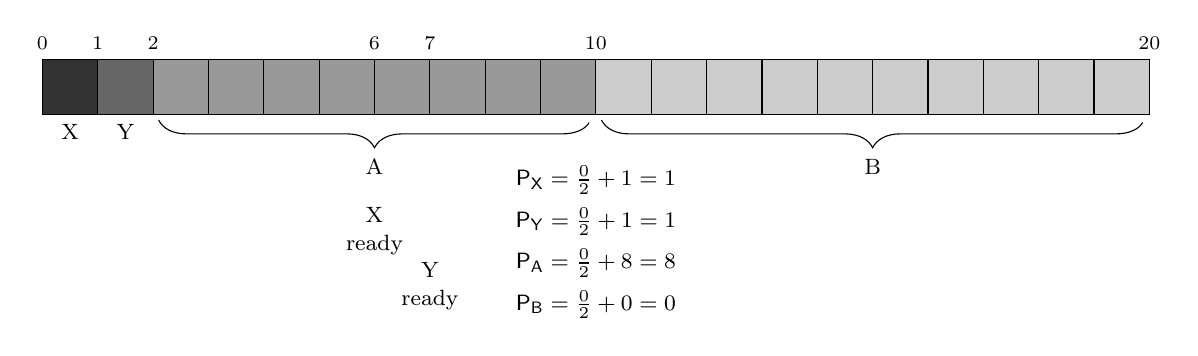
\begin{tikzpicture}

        \fill [black!80, visible on=<2->] (0,0) rectangle (2em, 2em);

        \fill [black!60, visible on=<3->] (2em,0) rectangle (4em, 2em);

        \fill [black!40, visible on=<4->] (4em,0) rectangle (20em, 2em);

        \fill [black!20, visible on=<8->] (20em,0) rectangle (40em, 2em);

        \draw (0,0) rectangle (40em,2em);

        \foreach \i in {1,...,19} {
          \draw [shorten >=0] (\i * 2em, 0) -- (\i * 2em, 2em);
        }

        \node [anchor=south] at (0em, 2em) {\scriptsize 0};
        \node [anchor=south, visible on=<2->] at (2em, 2em) {\scriptsize 1};
        \node [anchor=south, visible on=<3->] at (4em, 2em) {\scriptsize 2};
        \node [anchor=south, visible on=<5->] at (12em, 2em) {\scriptsize 6};
        \node [anchor=south, visible on=<6->] at (14em, 2em) {\scriptsize 7};
        \node [anchor=south] at (20em, 2em) {\scriptsize 10};
        \node [anchor=south] at (40em, 2em) {\scriptsize 20};

        \node [anchor=north, yshift=-3em, visible on=<5->] at (12em, 0em)
              {\footnotesize X};
        \node [anchor=north, yshift=-4em, visible on=<5->] at (12em, 0em)
              {\footnotesize ready};

        \node [anchor=north, yshift=-5em, visible on=<6->] at (14em, 0em)
              {\footnotesize Y};
        \node [anchor=north, yshift=-6em, visible on=<6->] at (14em, 0em)
              {\footnotesize ready};

        \node [anchor=north, yshift=-1.5em, visible on=<7->] at (20em, 0em)
              {\footnotesize $\mathsf{P_X} = \frac{0}{2} + 1 = 1$};
        \node [anchor=north, yshift=-3em, visible on=<7->] at (20em, 0em)
              {\footnotesize $\mathsf{P_Y} = \frac{0}{2} + 1 = 1$};
        \node [anchor=north, yshift=-4.5em, visible on=<7->] at (20em, 0em)
              {\footnotesize $\mathsf{P_A} = \frac{0}{2} + 8 = 8$};
        \node [anchor=north, yshift=-6em, visible on=<7->] at (20em, 0em)
              {\footnotesize $\mathsf{P_B} = \frac{0}{2} + 0 = 0$};

        \node [anchor=north, visible on=<2->] at (1em, 0) {\footnotesize X};

        \node [anchor=north, visible on=<3->] at (3em, 0) {\footnotesize Y};

        \draw [decorate, decoration={brace,amplitude=10pt,mirror,raise=2pt},
               visible on=<4->]
              (4.2em,0) -- (19.8em,0)
              node [midway, below, anchor=north, yshift=-1.25em]
              {\footnotesize A};

        \draw [decorate, decoration={brace,amplitude=10pt,mirror,raise=2pt},
               visible on=<8->]
              (20.2em,0) -- (39.8em,0)
              node [midway, below, anchor=north, yshift=-1.25em]
              {\footnotesize B};
      \end{tikzpicture}
    \end{center}
  \end{frame}

  \begin{frame}
    \frametitle{Now, Assume Processes A and B have a Priority of 6 (others are 0)}

    Assume we have 4 processes ready to execute arriving in order: X, Y, A, B
    
    \hspace{2em} A and B are CPU bound processes

    \hspace{2em} X and Y are I/O bound processes that execute for 0.1 s and
    block for 0.5 s
    
    Timer interrupts occur every 0.1 s, and each time slice is 1 s

    \vspace{2em}

    What is the scheduling? (each box is a timer interrupt)

    \vspace{-2em}

    \begin{center}
      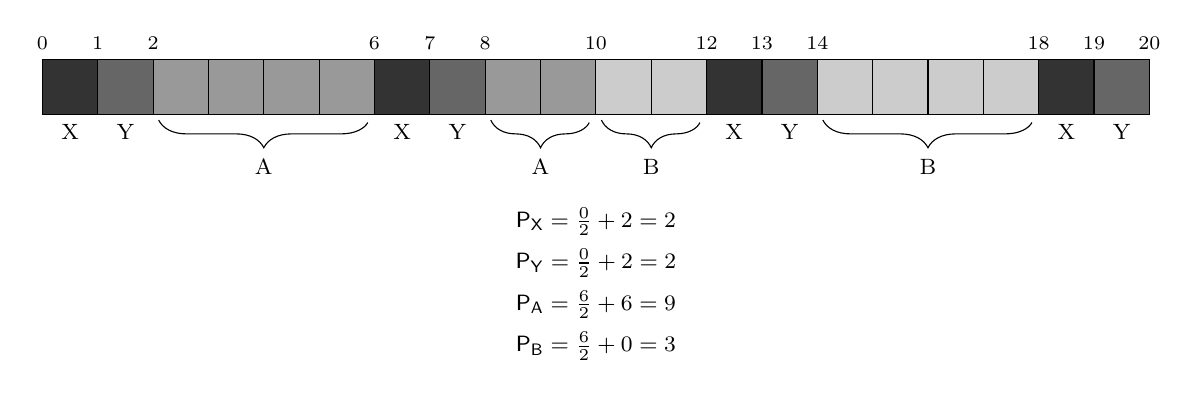
\begin{tikzpicture}

        \fill [black!80, visible on=<2->] (0,0) rectangle (2em, 2em);
        \fill [black!60, visible on=<3->] (2em,0) rectangle (4em, 2em);
        \fill [black!40, visible on=<4->] (4em,0) rectangle (12em, 2em);
        \fill [black!80, visible on=<5->] (12em,0) rectangle (14em, 2em);
        \fill [black!60, visible on=<6->] (14em,0) rectangle (16em, 2em);
        \fill [black!40, visible on=<7->] (16em,0) rectangle (20em, 2em);
        \fill [black!20, visible on=<9->] (20em,0) rectangle (24em, 2em);
        \fill [black!80, visible on=<10->] (24em,0) rectangle (26em, 2em);
        \fill [black!60, visible on=<11->] (26em,0) rectangle (28em, 2em);
        \fill [black!20, visible on=<12->] (28em,0) rectangle (36em, 2em);
        \fill [black!80, visible on=<13->] (36em,0) rectangle (38em, 2em);
        \fill [black!60, visible on=<14->] (38em,0) rectangle (40em, 2em);

        \draw (0,0) rectangle (40em,2em);

        \foreach \i in {1,...,19} {
          \draw [shorten >=0] (\i * 2em, 0) -- (\i * 2em, 2em);
        }

        \node [anchor=south] at (0em, 2em) {\scriptsize 0};
        \node [anchor=south, visible on=<2->] at (2em, 2em) {\scriptsize 1};
        \node [anchor=south, visible on=<3->] at (4em, 2em) {\scriptsize 2};
        \node [anchor=south, visible on=<4->] at (12em, 2em) {\scriptsize 6};
        \node [anchor=south, visible on=<5->] at (14em, 2em) {\scriptsize 7};
        \node [anchor=south, visible on=<6->] at (16em, 2em) {\scriptsize 8};
        \node [anchor=south, visible on=<9->] at (24em, 2em) {\scriptsize 12};
        \node [anchor=south, visible on=<10->] at (26em, 2em) {\scriptsize 13};
        \node [anchor=south, visible on=<11->] at (28em, 2em) {\scriptsize 14};
        \node [anchor=south, visible on=<12->] at (36em, 2em) {\scriptsize 18};
        \node [anchor=south, visible on=<13->] at (38em, 2em) {\scriptsize 19};
        \node [anchor=south] at (20em, 2em) {\scriptsize 10};
        \node [anchor=south] at (40em, 2em) {\scriptsize 20};

        \node [anchor=north, yshift=-3em, visible on=<8->] at (20em, 0em)
              {\footnotesize $\mathsf{P_X} = \frac{0}{2} + 2 = 2$};
        \node [anchor=north, yshift=-4.5em, visible on=<8->] at (20em, 0em)
              {\footnotesize $\mathsf{P_Y} = \frac{0}{2} + 2 = 2$};
        \node [anchor=north, yshift=-6em, visible on=<8->] at (20em, 0em)
              {\footnotesize $\mathsf{P_A} = \frac{6}{2} + 6 = 9$};
        \node [anchor=north, yshift=-7.5em, visible on=<8->] at (20em, 0em)
              {\footnotesize $\mathsf{P_B} = \frac{6}{2} + 0 = 3$};

        \node [anchor=north, visible on=<2->] at (1em, 0) {\footnotesize X};

        \node [anchor=north, visible on=<3->] at (3em, 0) {\footnotesize Y};

        \draw [decorate, decoration={brace,amplitude=10pt,mirror,raise=2pt},
               visible on=<4->]
              (4.2em,0) -- (11.8em,0)
              node [midway, below, anchor=north, yshift=-1.25em]
              {\footnotesize A};

        \node [anchor=north, visible on=<5->] at (13em, 0) {\footnotesize X};

        \node [anchor=north, visible on=<6->] at (15em, 0) {\footnotesize Y};

        \draw [decorate, decoration={brace,amplitude=10pt,mirror,raise=2pt},
               visible on=<7->]
              (16.2em,0) -- (19.8em,0)
              node [midway, below, anchor=north, yshift=-1.25em]
              {\footnotesize A};

        \draw [decorate, decoration={brace,amplitude=10pt,mirror,raise=2pt},
               visible on=<9->]
              (20.2em,0) -- (23.8em,0)
              node [midway, below, anchor=north, yshift=-1.25em]
              {\footnotesize B};

        \node [anchor=north, visible on=<10->] at (25em, 0) {\footnotesize X};

        \node [anchor=north, visible on=<11->] at (27em, 0) {\footnotesize Y};

        \draw [decorate, decoration={brace,amplitude=10pt,mirror,raise=2pt},
               visible on=<12->]
              (28.2em,0) -- (35.8em,0)
              node [midway, below, anchor=north, yshift=-1.25em]
              {\footnotesize B};

        \node [anchor=north, visible on=<13->] at (37em, 0) {\footnotesize X};

        \node [anchor=north, visible on=<14->] at (39em, 0) {\footnotesize Y};
      \end{tikzpicture}
    \end{center}
  \end{frame}

  \begin{frame}[fragile]
    \frametitle{We'll Explore Multi-Level Page Tables Live}

    See: \lstinline!examples/lecture-23!

    \vspace{2em}

    To build, in the \lstinline!lecture-23! directory do:

    \begin{lstlisting}
meson setup build
cd build
meson compile
./mmusim
    \end{lstlisting}
  \end{frame}
\end{document}
